\chapter{Diagramme des cas d'utilisation}

L'étape de modélisation dans le cadre d'un projet informatique est l'étape la plus importante.
Se lancer tête baissée dans la programmation n'est pas une solution viable pour un projet
de grande ampleur car il faudra revenir sur le code déjà produit, c'est donc une perte de
temps. Il vaut mieux prendre le temps de réfléchir à ce que l'on cherche à créer, à comment
réaliser le projet, comment seront stockées les données, etc.

La phase d'analyse ne doit donc surtout pas être prise à la légère, au risque de se retrouver
avec du code impossible à maintenir, ou finalement inutile, car il sera à revoir plusieurs fois.

    \begin{figure}[h]
        \begin{center}
            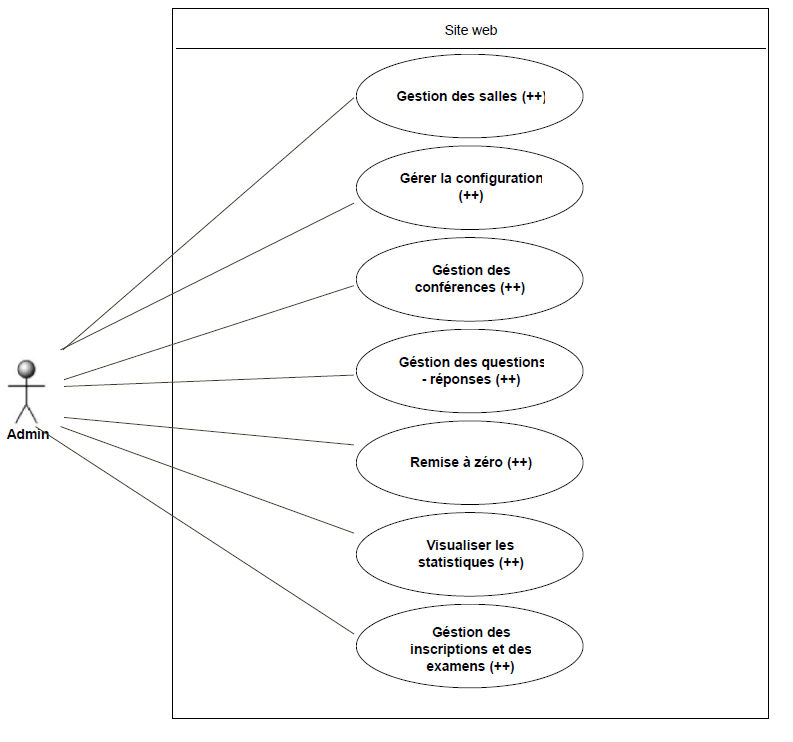
\includegraphics[scale=0.85]{images/uml/adminMenu.png} 
        \end{center}

        \caption{Administrateur menu}
        \label{a=Administrateur menu}
    \end{figure}

    \begin{figure}[h]
        \begin{center}
            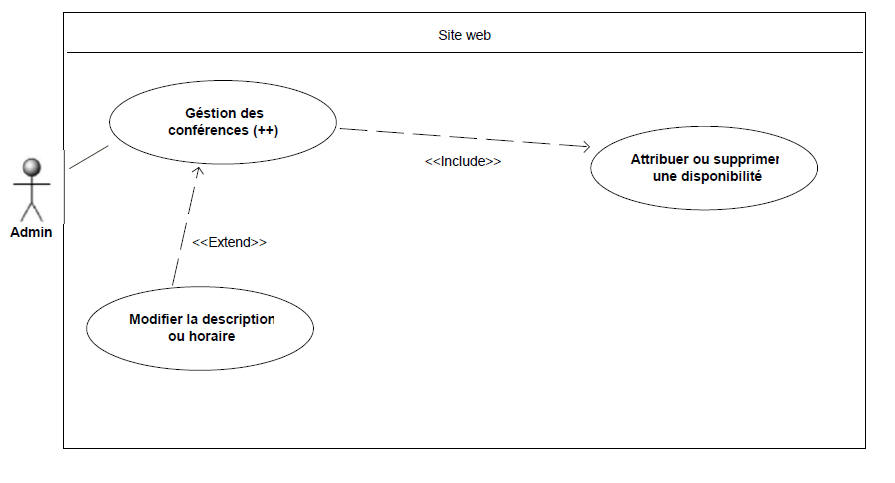
\includegraphics[scale=0.75]{images/uml/adminConference.png} 
        \end{center}

        \caption{Administrateur conference}
        \label{Administrateur conference}
    \end{figure}

    \begin{figure}[h]
        \begin{center}
            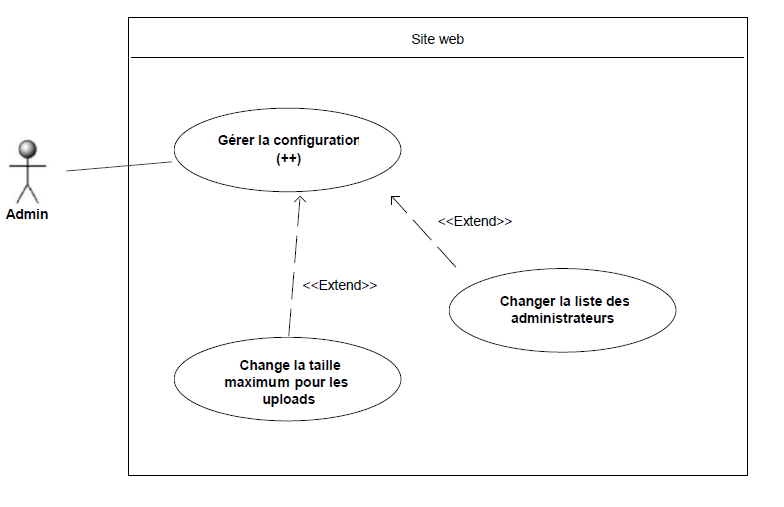
\includegraphics[scale=0.85]{images/uml/adminConfiguration.png} 
        \end{center}

        \caption{Administrateur configuration}
        \label{Administrateur configuration}
    \end{figure}

    \begin{figure}[h]
        \begin{center}
            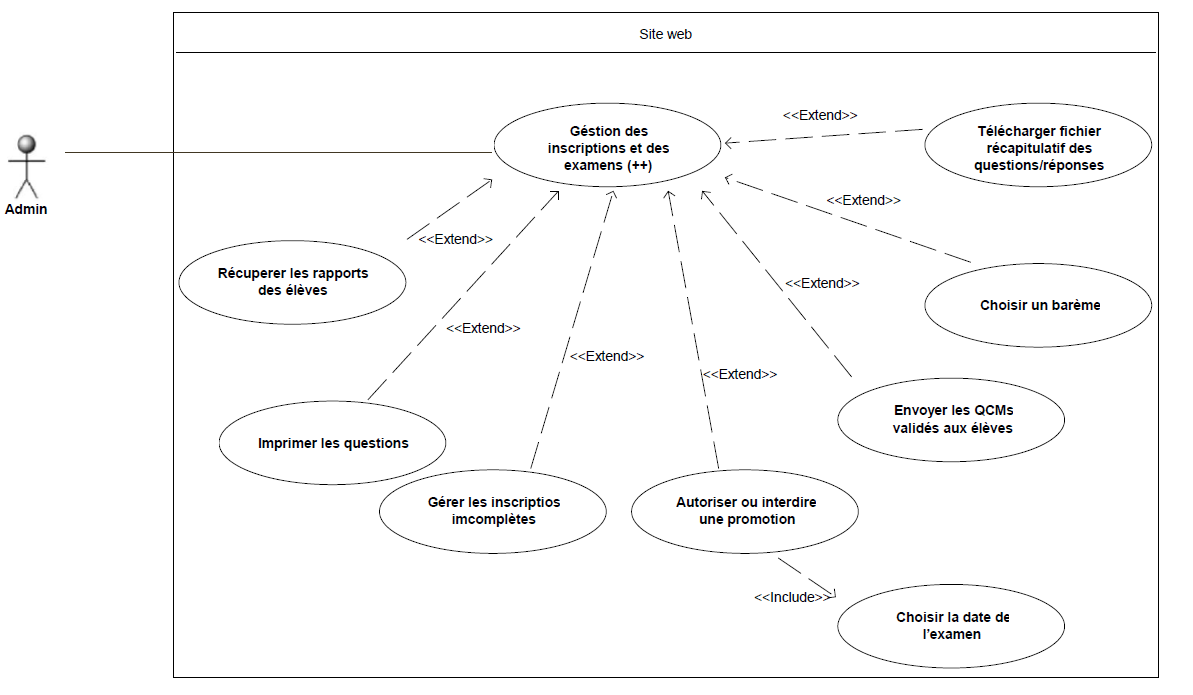
\includegraphics[width=18cm,height=15cm, angle=90]{images/uml/adminInscriptionsExamens.png} 
        \end{center}

        \caption{Administrateur inscription}
        \label{Administrateur inscription}
    \end{figure}

    \begin{figure}[h]
        \begin{center}
            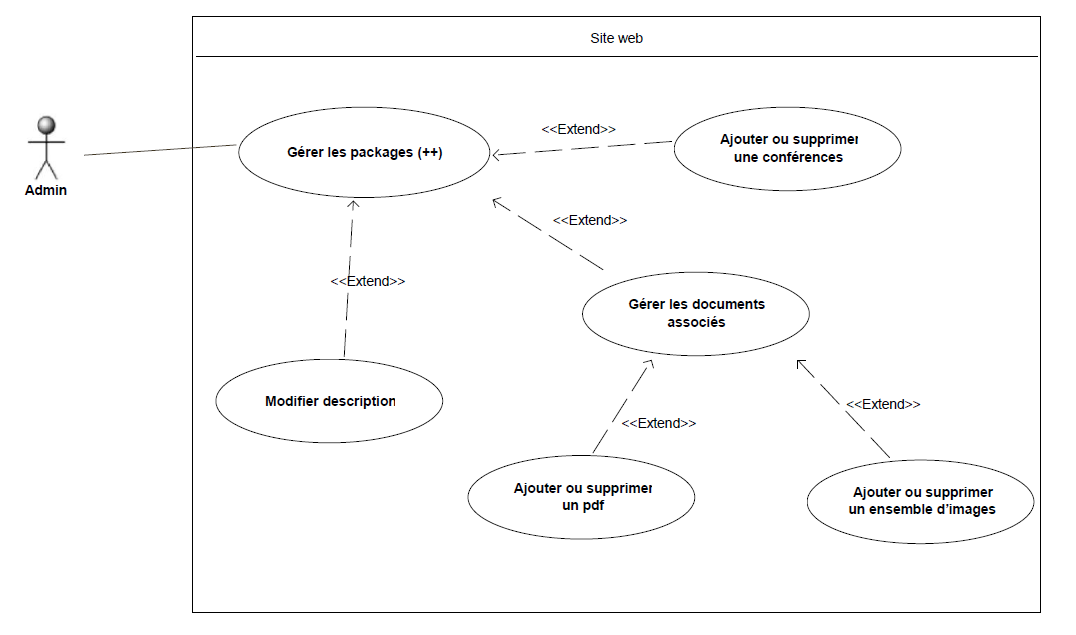
\includegraphics[scale=0.65]{images/uml/adminPackages.png} 
        \end{center}

        \caption{Administrateur packages}
        \label{Administrateur packages}
    \end{figure}

    \begin{figure}[h]
        \begin{center}
            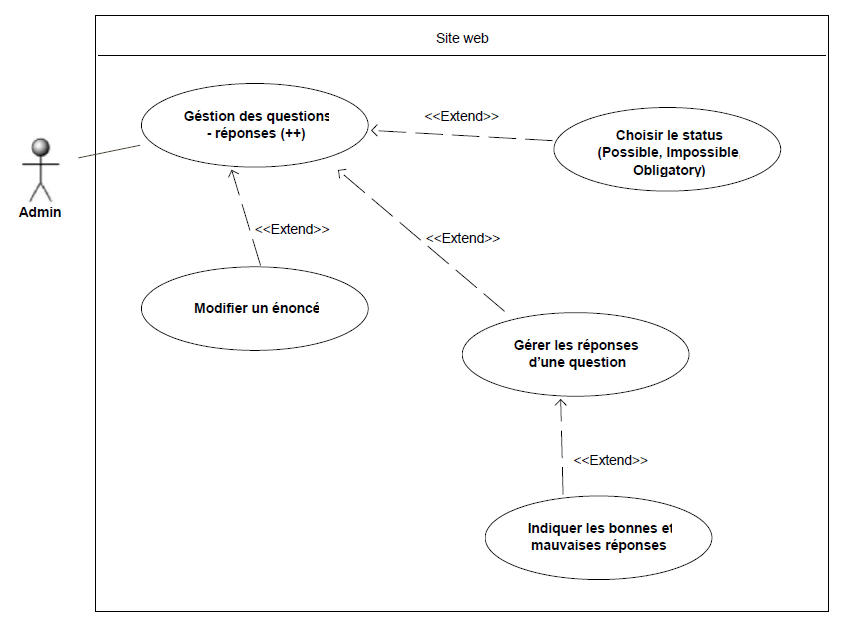
\includegraphics[scale=0.70]{images/uml/adminQuestionsReponses.png} 
        \end{center}

        \caption{Administateur questions et réponses}
        \label{Administateur questions et réponses}
    \end{figure}

    \begin{figure}[h]
        \begin{center}
            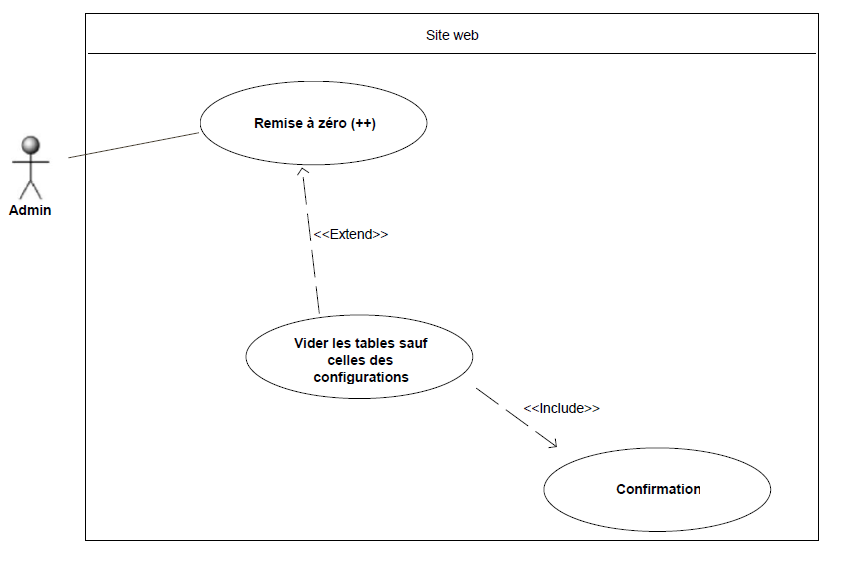
\includegraphics[scale=0.70]{images/uml/adminRAZ.png} 
        \end{center}

        \caption{Administateur remise à zéro}
        \label{Administateur remise à zéro}
    \end{figure}

    \begin{figure}[h]
        \begin{center}
            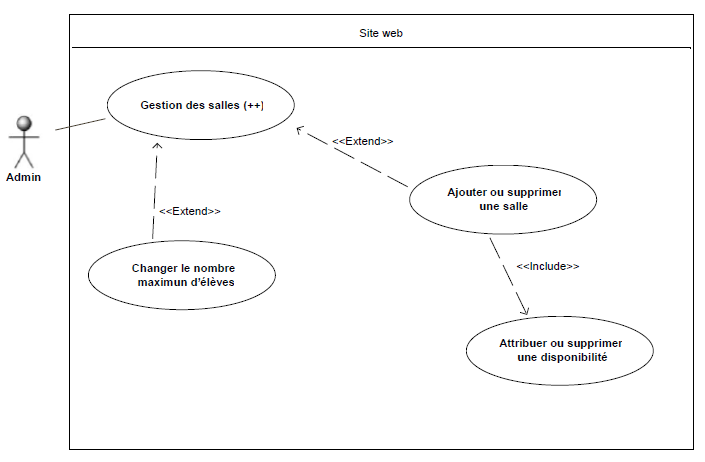
\includegraphics[scale=0.70]{images/uml/adminSalles.png} 
        \end{center}

        \caption{Administrateur salles}
        \label{Administrateur salles}
    \end{figure}

    \begin{figure}[h]
        \begin{center}
            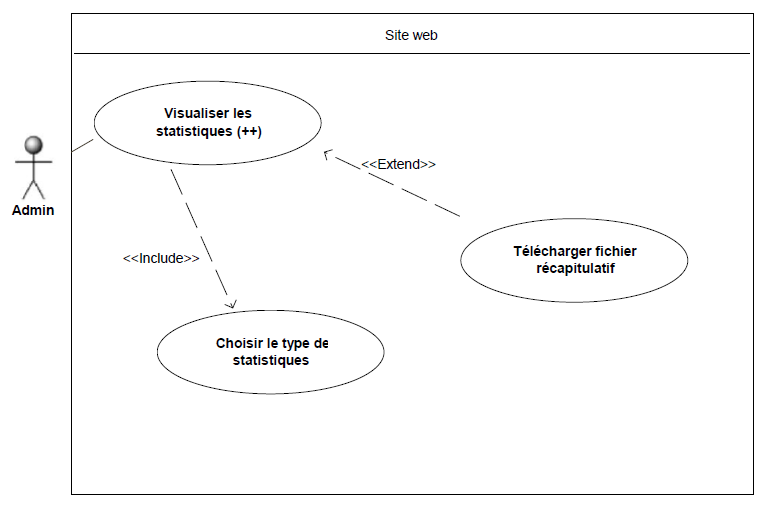
\includegraphics[scale=0.70]{images/uml/adminStats.png} 
        \end{center}

        \caption{Administrateur statistiques}
        \label{Administrateur statistiques}
    \end{figure}

    \begin{figure}[h]
        \begin{center}
            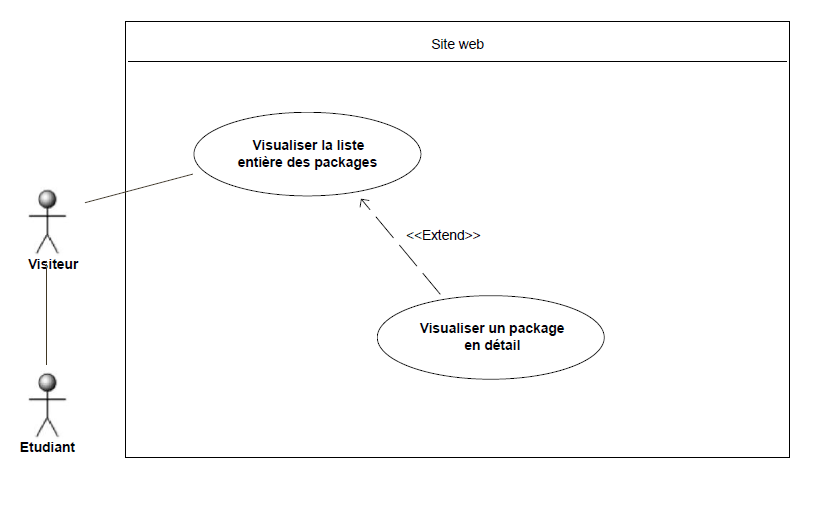
\includegraphics[scale=0.70]{images/uml/visiteurMenu.png} 
        \end{center}

        \caption{Visiteur menu}
        \label{Visiteur menu}
    \end{figure}

    \begin{figure}[h]
        \begin{center}
            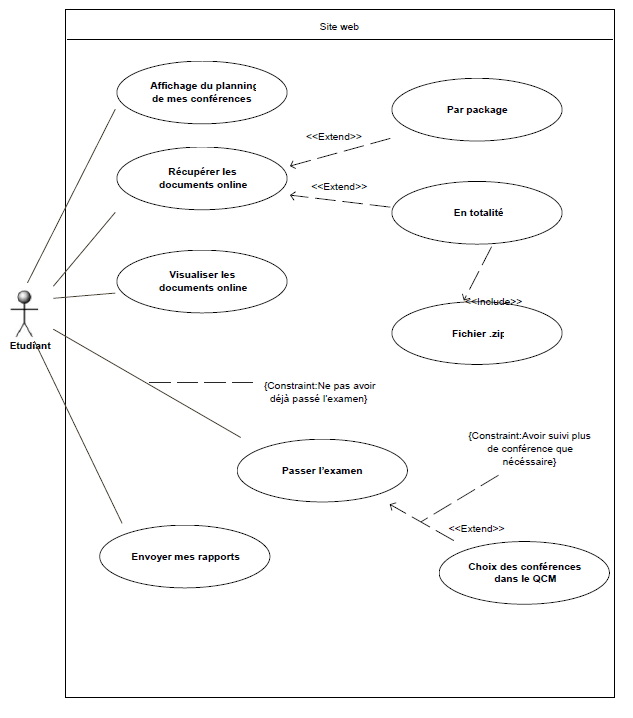
\includegraphics[scale= 0.70]{images/uml/etudiantMenuFinal.png} 
        \end{center}

        \caption{Etudiant menu final}
        \label{Etudiant menu final}
    \end{figure}

    \begin{figure}[h]
        \begin{center}
            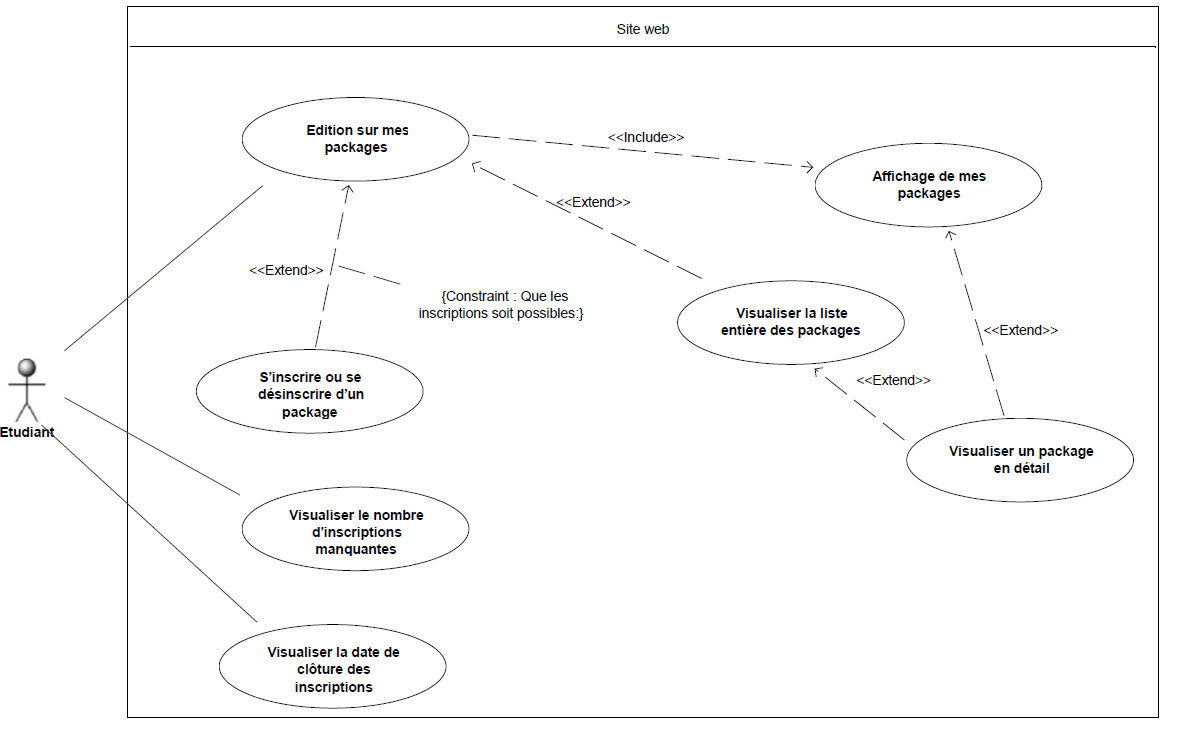
\includegraphics[height=14cm,width=15cm]{images/uml/etudiantMenuInitial.png} 
        \end{center}

        \caption{Etudiant menu initial}
        \label{Etudiant menu initial}
    \end{figure}






\chapter{Diagrammes de classes}
    Cette annexe fait suite à celle concernant les cas d'utilisations. Elle est 
toute aussi importante afin de garder un ensemble cohérent.

    Les pages suivantes contiennent les diagrammes de classes du framework du site
web.

    \begin{figure}[h]
        \begin{center}
            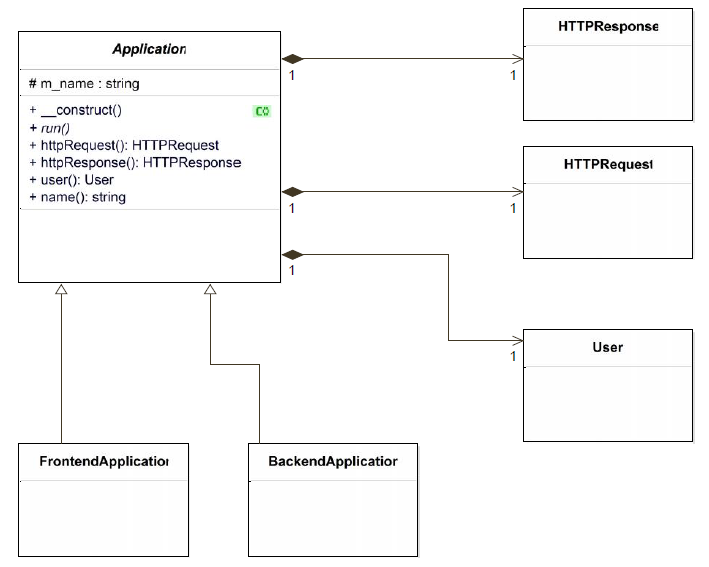
\includegraphics[scale=0.9]{images/uml/classes/Application.png} 
        \end{center}

        \caption{Classe Application}
        \label{Classe Application}
    \end{figure}


    \begin{figure}[h]
        \begin{center}
            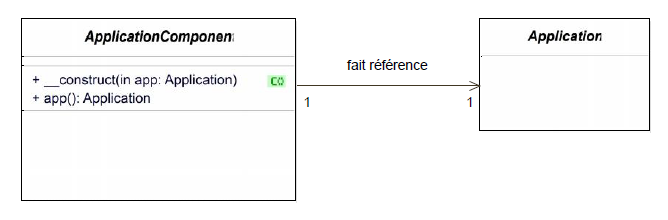
\includegraphics[scale=1.0]{images/uml/classes/ApplicationComponent.png} 
        \end{center}

        \caption{Classe ApplicationComponent}
        \label{Classe ApplicationComponent}
    \end{figure}


    \begin{figure}[h]
        \begin{center}
            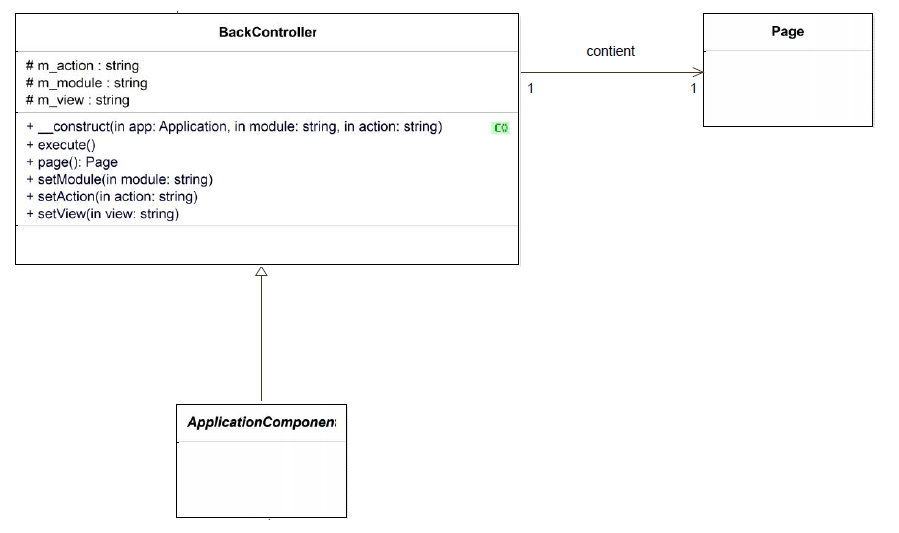
\includegraphics[scale=0.7]{images/uml/classes/BackController.png} 
        \end{center}

        \caption{Classe BackController}
        \label{Classe BackController}
    \end{figure}


    \begin{figure}[h]
        \begin{center}
            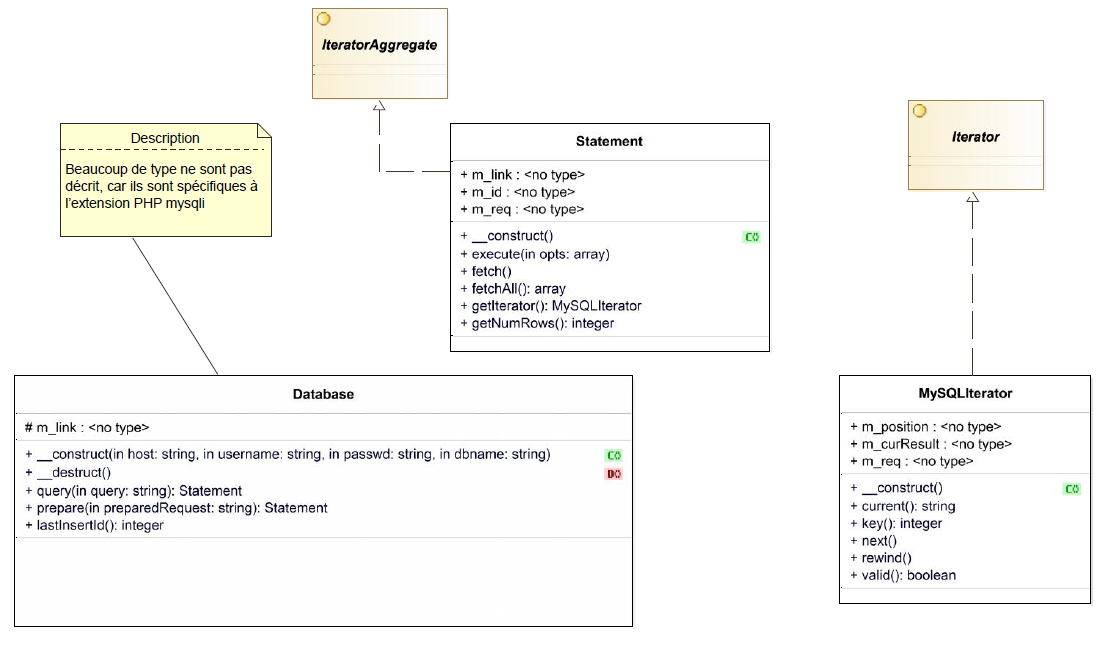
\includegraphics[angle=90, scale=0.8]{images/uml/classes/Database.png} 
        \end{center}

        \caption{Classe Database}
        \label{Classe Database}
    \end{figure}


    \begin{figure}[h]
        \begin{center}
            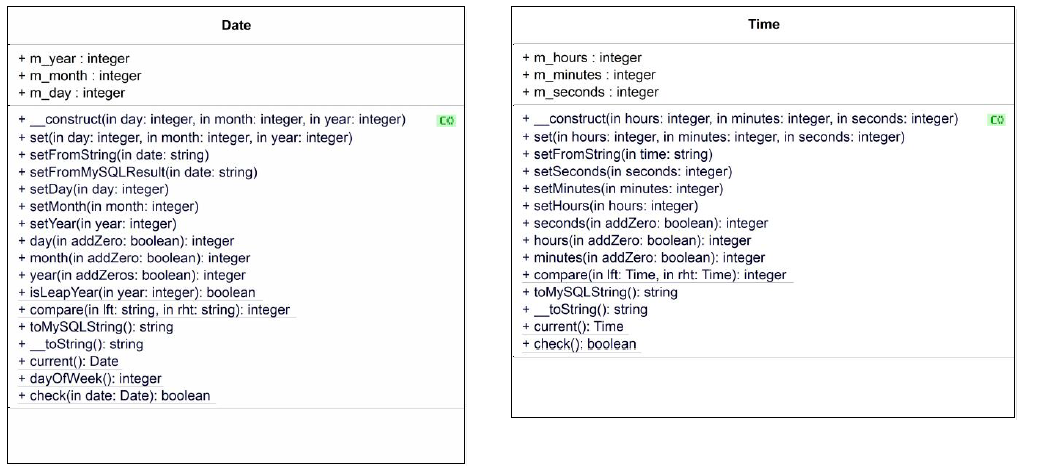
\includegraphics[angle=90, scale=0.8]{images/uml/classes/DateTime.png} 
        \end{center}

        \caption{Classe DateTime}
        \label{Classe DateTime}
    \end{figure}


    \begin{figure}[h]
        \begin{center}
            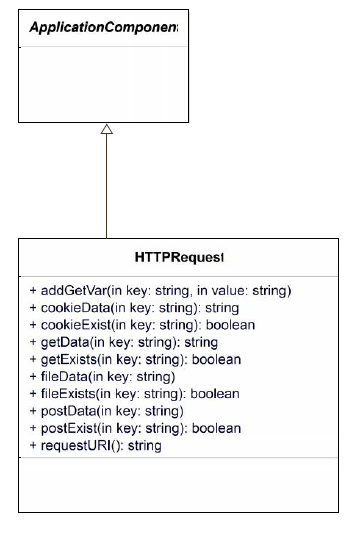
\includegraphics[scale=1.0]{images/uml/classes/HTTPRequest.png} 
        \end{center}

        \caption{Classe HTTPRequest}
        \label{Classe HTTPRequest}
    \end{figure}


    \begin{figure}[h]
        \begin{center}
            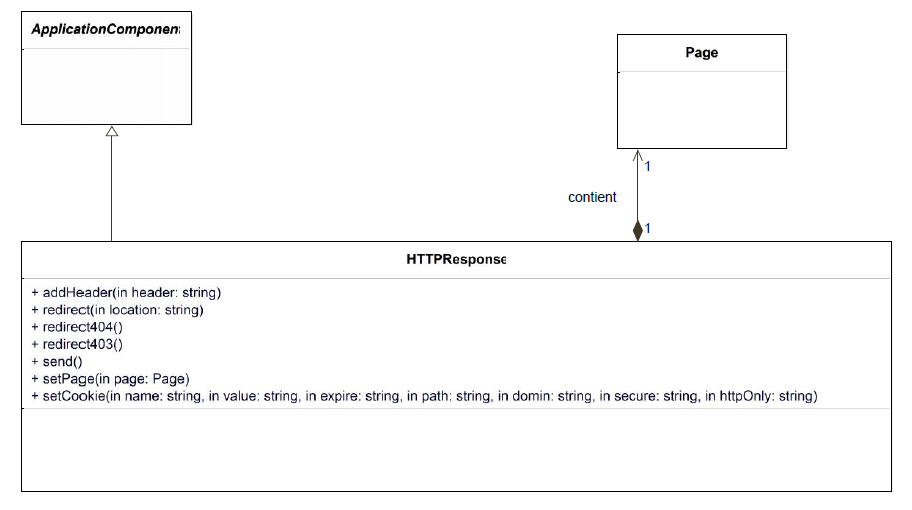
\includegraphics[angle=90, scale=0.8]{images/uml/classes/HTTPResponse.png} 
        \end{center}

        \caption{Classe HTTPResponse}
        \label{Classe HTTPResponse}
    \end{figure}


    \begin{figure}[h]
        \begin{center}
            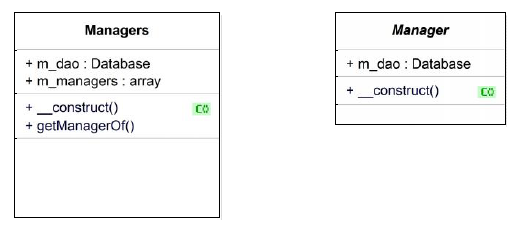
\includegraphics[scale=1.0]{images/uml/classes/Manager.png} 
        \end{center}

        \caption{Classe Manager}
        \label{Classe Manager}
    \end{figure}


    \begin{figure}[h]
        \begin{center}
            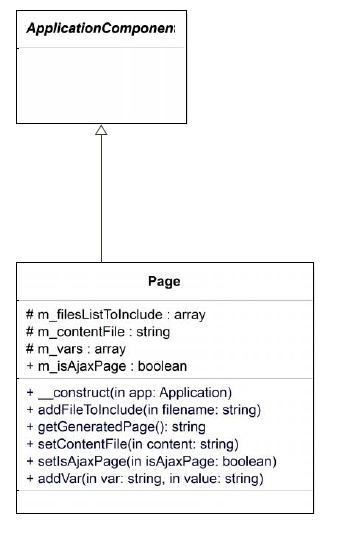
\includegraphics[scale=1.0]{images/uml/classes/Page.png} 
        \end{center}

        \caption{Classe Page}
        \label{Classe Page}
    \end{figure}


    \begin{figure}[h]
        \begin{center}
            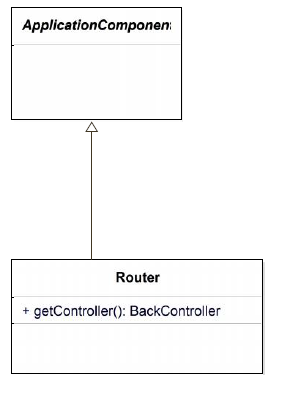
\includegraphics[scale=1.0]{images/uml/classes/Router.png} 
        \end{center}

        \caption{Classe Router}
        \label{Classe Router}
    \end{figure}


    \begin{figure}[h]
        \begin{center}
            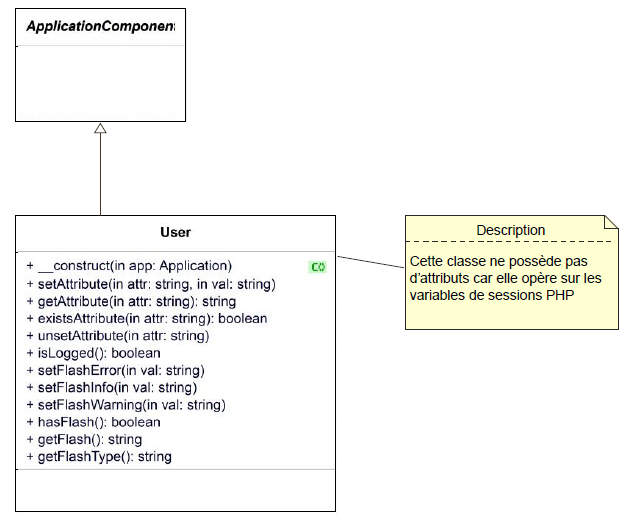
\includegraphics[scale=1.0]{images/uml/classes/User.png} 
        \end{center}

        \caption{Classe User}
        \label{Classe User}
    \end{figure}
